\newcommand{\sheetnum}{%
	04
}
%\setcounter{section}{\sheetnum-3}
\newcommand{\tutorialtitle}{%
    Gradient methods for parameter optimization
}
\newcommand{\tutorialtitleshort}{%
	Gradient methods
}
% for slides
\subtitle{\sheetnum \tutorialtitle}

\maxdeadcycles=1000 % Workaround for ! Output loop---100 consecutive dead cycles because of too many figures

% The following use of algroithms does not work well with the notes:
%
%
%
%
% instead use the following for your algorithms:
%
%\begin{figure}[!t]
%\removelatexerror
%\begin{algorithm}[H]
    % your algo here
    %\label{alg:algolabel}
    %\caption{algocaption}
%\end{algorithm}
%\end{figure}
%\begin{algorithm}
% Below is the definition for the command \removelatexerror:
\makeatletter
\newcommand{\removelatexerror}{\let\@latex@error\@gobble}
\makeatother

\begin{document} %%%%%%%%%%%%%%%%%%%%%%%%%%%%%%%%%%%%%%%%%%%%%%%%%%%%%%%

\sheet{\sheetnum}{\tutorialtitleshort}

\ttopic{\tutorialtitle}

\columnratio{0.2,0.8}\textbf{}
\begin{paracol}{2}
%\setlength{\columnseprule}{0.1pt}
%\setlength{\columnsep}{5em}

\begin{rightcolumn}

% notes version will ignore it
\begin{frame}
\titlepage
\end{frame}

\begin{frame}
\tableofcontents
\end{frame}


\mode<all>
\section{Linear neuron for regression: analytical solution}

\subsection{Data, Model and Objective}

\begin{frame}\frametitle{Setting}

\underline{Data}:\\

\begin{align*}
\text{observations} \quad x &\in \R \\
\text{label}        \quad y_{T} &\in \R \\
\text{Data set } &: \Big\{
\left(x^{(1)}, y_T^{(1)} 
\right)
\,,\, \ldots \,,\,
\left( x^{(\alpha)}, y_T^{(\alpha)} \right)
\,,\, \ldots \,,\, 
\left( x^{(p)}, y_T^{(p)} \right) 
\Big\}
\end{align*}

\pause

\underline{Model}:\\

linear neuron:
\begin{equation}
    y(x; \vec w) = w_{0} + w_{1} x = \vec w^{\top} \vec x
\end{equation}

with $\vec x := (1, x)^{\top} \in \R^{2}$ and $\vec w := (w_{0}, w_{1})^{\top} \in \R^{2}$

\end{frame}

\begin{frame}

\underline{Cost function}:\\

Quadratic error

\begin{align}
E^{T} &= \frac{1}{p} \sum_{\alpha=1}^{p} \;
\frac{1}{2} \, \left( y(x^{(\alpha)}; \vec w)- y^{(\alpha)}_{T}\right)^{2}\\
&= \frac{1}{p} \sum_{\alpha=1}^{p}
\;e^{(\alpha)}
\end{align}

\mode<article>{
The term $\frac{1}{2}$ is merely for convinience when computing the gradient later.
}

\pause

\underline{Optimization}:\\

\begin{align}
E^{T} &\eqexcl \min_{\vec w}\\
\frac{\partial E^{T}}{\partial \vec w} &= \vec 0 \qquad\qquad \text{(satisfied by extrema)}
\label{eq:extremacond}
\end{align}
    
\end{frame}

\newpage

\subsection{Calculating the gradient}

%\mode<article>{
%Finding extrema that satisfy \eqref{eq:extremacond}:
%}

\begin{frame}\frametitle{\subsecname}
 
% temporarily change footnote marks to symbols so not to confuse with exponents
\renewcommand*{\thefootnote}{\fnsymbol{footnote}}    

\begin{align}
\frac{\partial E^{T}}{\partial \vec w} 
\;\;&=\;\; 
\frac{1}{p} \sum_{\alpha=1}^{p} \; 
\frac{\partial e^{(\alpha)}}{\partial \vec w}\\
\;\;&\stackrel{\mathclap{
\substack{\text{chain}\\\text{rule}}}
}
{=}\;\;
\frac{1}{p} \sum_{\alpha=1}^{p} \;
{\color{blue}
\frac{\partial e^{(\alpha)}}{\partial y(x^{(\alpha)};\vec w)}
} 
\cdot
{\color{orange}
\frac{\partial y(x^{(\alpha)};\vec w)}{\partial \vec w}
}\\
\;\;&=\;\;
\frac{1}{p} \sum_{\alpha=1}^{p} \;
{\color{blue}
\big( y(x^{(\alpha)}; \vec w) - y_{T}^{(\alpha)} \big)
}
\cdot
{\color{orange}
\frac{\partial}{\partial \vec w} \vec w^{\top} \vec x^{(\alpha)}
}
\;\footnotemark \\
\;\;&=\;\;
\frac{1}{p} \sum_{\alpha=1}^{p} \;
{\color{blue}
\big( \vec w^{\top}\vec x^{(\alpha)} - y_{T}^{(\alpha)} \big)
}
\cdot
{\color{orange}
\vec x^{(\alpha)}
}\\
\;\;&=\;\;
\frac{1}{p} \sum_{\alpha=1}^{p} \;
{\color{orange}
\vec x^{(\alpha)}
}
\cdot
{\color{blue}
\big( {\vec x^{(\alpha)}}^{\top}\vec w - y_{T}^{(\alpha)} \big)
}\;\footnotemark \\
\;\;&=\;\;
\frac{1}{p} \sum_{\alpha=1}^{p} \;
\Big( 
\vec x^{(\alpha)}
\left({\vec x^{(\alpha)}}^{\top}\right)\vec w - \vec x^{(\alpha)} y_{T}^{(\alpha)}
\Big)\\
\;\;&=:\;\; \vec g
\end{align}    

%\notesonly{ 
\footnotetext{
partial derivative calculated by using 
$y(x^{(\alpha)};\vec w) = \vec w^{\top}\vec x^{(\alpha)}$ and 
$\frac{\partial}{\partial \vec a}\left(\vec a^{\top} \vec b\right) = \vec b = (b_{1}, b_{2}, \ldots, b_{N})^{\top}$
}
\footnotetext{
$\vec w^{\top}\vec x^{(\alpha)} = {\vec x^{(\alpha)}}^{\top} \vec w$
}
%}

% change footnote marks back to original scheme (numbers)
\renewcommand*{\thefootnote}{\arabic{footnote}}

\end{frame}

\subsection{Finding minimia}

\begin{frame}\frametitle{\subsecname}

Computing the Hessian $\vec H$ to identify minima among the solutions that satisfy \eqref{eq:extremacond}:

Let $\vec g$ denote the gradient vector: $\vec g = \frac{\partial E^{T}}{\partial \vec w}$

\begin{align}
\vec H := \frac{\partial \vec g}{\partial \vec w}
\;\;&=\;\;
\frac{1}{p} \sum_{\alpha=1}^{p} \;
\frac{\partial}{\partial \vec w}
\left(
\frac{e^{(\alpha)}}{y(\vec x^{(\alpha)}; \vec w)}
\cdot
\frac{\partial y(x^{(\alpha)};\vec w)}{\partial \vec w} 
\right)\\
\;\;&=\;\;
\frac{1}{p} \sum_{\alpha=1}^{p} \;
\frac{\partial}{\partial \vec w}
\Big( 
\vec x^{(\alpha)}
\left({\vec x^{(\alpha)}}^{\top}\right) \vec w 
\;-\; 
\underbrace{
\vec x^{(\alpha)}
y_{T}^{(\alpha)} 
}_{\text{indep. of }\vec w}
\Big)\\
\end{align}

\end{frame}

\mode*

\clearpage

\mode<all>
\section{Gradient methods}

\subsection{The need for gradient-based optimization}

\begin{frame}


\notesonly{
We have some cost function we want to minimize but solving the problem analytically is not applicable.

}



\question{In what case(s) do we avoid an analytical solution?}

\pause
\begin{itemize}
	\item We cannot fit all the data into memory.
	\item It involves finding an inverse of a matrix, that is not invertible (e.g. linear regression $(\vec X \, \vec X^\top)^{-1}\vec X \, \vec y_{True}^\top$.
	\item There is no closed-form solution for the model we're using (e.g. MLP)
	\item Computing the Hessian is too costly. Newton's method also not applicable.\notesonly{\footnote{
	Newton's method finds the root of a function iteratively using the second-order Taylor expansion of the cost function around a point $\vec w_t$. For more details see Haykin Ch. 3.3.
	}}
	\item Non-stationary data. We cannot easily adapt to changes over time.
\end{itemize}

\end{frame}

We therefore opt for Gradient-based optimization which is an iterative optimization procedure. 
In the case of a \emph{minimization} problem one can reduce some cost function $E^T_{[\vec w]}$ by taking steps in the direction of steepest \emph{descent}.
For minimizing some cost function $E^T_{[\vec w]}$ w.r.t. to a set of weights $\vec w$, it follows that, if

\begin{equation}
\vec w_{t+1} = \vec w_t - \underbrace{\eta_t \, \frac{\partial E^T}{\partial \vec w} \Bigg|_{\vec w_t}}_{\text{update}~\Delta \vec w}
\end{equation}

and a small enough $\eta_t \in \R^+$, then the cost at the next step $t+1$ will become less or remain unchanged. That is $E^T_{[\vec w_{t+1}]} \le E^T_{[\vec w_{t}]}$.
We refer to $\eta_t$ as the learning rate. It allows us to control the size of the step we take in the direction of the gradient.
\emph{Subtracting} the gradient from the current $\vec w_t$ lets us move against the slope in towards some minimum. 

The behavior of gradient descent can be controlled by modulating 
\begin{itemize}
\item The ``scope'' of the gradient. What do we use for deciding on the direction of the update?
\item The learning rate schedule. How big of a step do we take in the direction of the gradient?
\end{itemize}


\subsection{``Scope'' of the gradient}

The scope of the gradient method refers to the amount of data used for deciding on the direction of the gradient.


\begin{frame}

\renewcommand*{\arraystretch}{1.}{
\begin{table}[h]
\begin{tabular}[c]{r|l|l}
\hline
batch      & 
$\displaystyle
\frac{\partial E^{T}}{\partial \vec w} 
\;=\;
\frac{1}{p} \sum_{\alpha=1}^{p} 
\frac{\partial e^{(\alpha)}}{\partial \vec w}
$ &
\pause
\\[10mm]
\hline
mini-batch & \begin{tabular}[c]{@{}c@{}}
$\displaystyle
\frac{\partial E^{T}}{\partial \vec w} 
\;\approx\;
\frac{1}{|\mathcal{M}|} \sum_{\beta \in \mathcal{M}}^{|\mathcal{M}|} 
\frac{\partial e^{(\beta)}}{\partial \vec w}
$\\
$|\mathcal{M}| \ll p$\\
where $\mathcal{M}$ is a set of indices\\
 sampled randomly \\
 from 
 $\{1,\ldots,p\}$
\end{tabular} 
&
\begin{tabular}[c]{@{}l@{}}
noisy \\
estimate of $E^T$, \\
becomes less noisy with \\
larger $|\mathcal{M}|$
\end{tabular} 
\pause
\\[10mm]
\hline
online     &
\begin{tabular}[c]{@{}c@{}}
$\displaystyle
\frac{\partial E^{T}}{\partial \vec w} 
\;\approx\;
\frac{\partial e^{(\beta)}}{\partial \vec w}
$\\
a single random\\ data point $(\vec x^{(\beta)}, \vec y_T^{(\beta)})$
\end{tabular}    &
\begin{tabular}[c]{@{}l@{}}
very noisy \\
estimate of $E^T$
\end{tabular}\\
\end{tabular}
\end{table}
}

\end{frame}


\subsection{Learning rate schedules}

\mode*

\clearpage

\mode<all>
\subsection{The Conjugate gradient method}

\subsubsection{Motivation}

\notesonly{
We have seen how line search allows us to reach the minimum along the direction of the gradient $\vec g_t$ computed at time step $t$. It achieves this by manipulating the magnitude of the step we take towards a lower cost.
Looking at what happens over multiple time steps we observe the following movements on the surface of the cost function:
}
\begin{frame}{Limitations of line search}

\begin{center}
	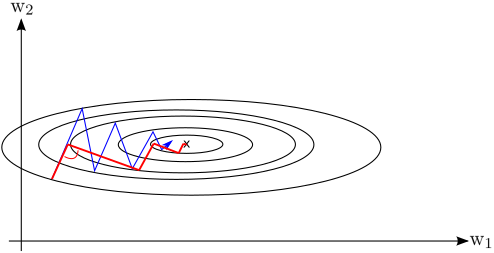
\includegraphics[width=0.6\textwidth]{img/section1_fig23_clean_ls}
	\captionof{figure}{Weight updates by following line search 
	%(\textcolor{red}{red}).}
	(red).}
\end{center}

\mode<presentation>{
	%\only<2>{
		%\begin{center}
			%\includegraphics[width=0.3\textwidth]{img/meme_point}
		%\end{center}
	%}
	%\only<3>{
		%\begin{center}
			%\includegraphics[width=0.3\textwidth]{img/meme_deeper}
		%\end{center}
	%}
	%\only<4>{
	\only<4>{
		\begin{center}
			\includegraphics[width=0.3\textwidth]{img/meme_direction}
		\end{center}
	}
}

\end{frame}

\begin{frame}{Limitations of line search}
		\begin{center}
			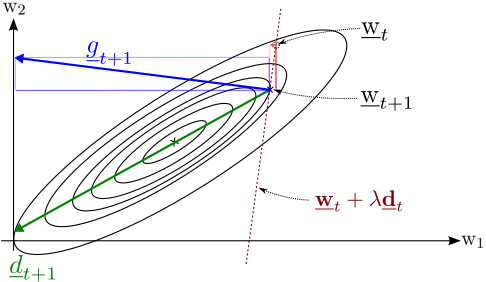
\includegraphics[width=0.8\textwidth]{img/conjugate_direction_c}
			\notesonly{
			\captionof{figure}{The conjugate direction avoids undoing progress made in the previous step.}
			}
		\end{center}
\end{frame}

\begin{frame}\frametitle{Conjugate gradient method}
\mode<article>{
\underline{Conjugate gradient method}:

}

		\begin{eqnarray}
			\vec{w}_{t+1}
			%& = & \mathrm{w}_{ij}(t) 
			%+ \Delta \mathrm{w}_{ij}(t)  \\ 
			& =&  \vec{w}_t + \eta_t \, \vec{d}_{t}
		\end{eqnarray}

Don't undo progress of previous search directions $\vec d_{t}$, $\vec d_{t-1}$.

In other words:

The component of the gradient parallel to the old direction $\vec d_{t}$ should
remain zero along the new direction $\vec d_{t+1}$

\pause
	
	\begin{block}{$ $}
		\textbf{Initialization:} $\vec{w},\quad \vec{d} = - \vec{g}$\\
		\vspace{3mm}

		\While{stopping criterion not fulfilled}{
			\vspace{1mm}
			Minimize $E^T$ along $\vec{d}$ using line-search 
				\quad $\rightarrow$ new $\vec{w}$ \\[1mm]
			Calculate the new conjugate direction 
				\quad $\;\,\rightarrow$ new $\vec{d}$
			\vspace{1mm}
		}
	\end{block}

\end{frame}

% -----------------------------------------------------------------------------
\begin{frame}\frametitle{Adaptive momentum: the Polak-Ribiere rule}
	\begin{equation}\tag{conjugate direction}
		\vec{d}_{t+1} = - 
		\overbrace{\frac{\partial E^T}{\partial \vec{w}}
			\bigg|_{\vec{w}_{t+1}}}^{\vec{g}_{t+1}} + \beta_t \, \vec{d}_t
	\end{equation}%\\[5mm]
	\begin{equation}\tag{``smart momentum''}
		\beta_t = \underbrace{ \frac{\vec{g}_{t+1}^\top
			\big( \vec{g}_{t+1} - \vec{g}_t \big)}{
			\vec{g}_t^\top \vec{g}_t} }_{
				\text{Polak-Ribiere rule}}
	\end{equation}
	OR
			  \begin{equation} %\tag{Fletcher-Reeves form}
		  		\beta_t = \underbrace{-\frac{\vec{g}_{t+1}^\top\vec{g}_{t+1}}%
		  		{\vec{g}_t^\top\vec{g}_t}}_{\text{Fletcher-Reeves}}.
		  \end{equation} 
	%\iitem{determine learning rate $\eta_t$ via line search}
\end{frame}

% -----------------------------------------------------------------------------
\begin{frame}\frametitle{Conjugate gradient descent algorithm}
\slidesonly{
	\begin{block}{$ $}
		\textbf{Initialization:} $\vec{w},\quad \vec{d} = - \vec{g}$\\
		\vspace{3mm}

		\While{stopping criterion not fulfilled}{
			\vspace{1mm}
			Minimize $E^T$ along $\vec{d}$ using line-search 
				\quad $\rightarrow$ new $\vec{w}$ \\[1mm]
			Calculate the new conjugate direction 
				\quad $\;\,\rightarrow$ new $\vec{d}$
			\vspace{1mm}
		}
	\end{block}
	}
	\iitem{Subsequent search directions lose conjugacy 
		\iitem{search direction should be reset to the 	steepest \\ 
			descent direction at least every $N$ iterations (in practice apply heuristic, e.g. reset every 5 steps)}
	}
\end{frame}

\slidesonly{
\begin{frame} \frametitle{Comparison}
\placeimage{0.5}{2.5}{img/section1_fig23_clean}{width=6cm}
\placeimage{8}{2.5}{img/section1_fig24_clean}{width=6cm}
\placeimage{0.5}{8.5}{img/section1_fig23_clean_ls}{width=6cm}
\placeimage{8}{8.5}{img/section1_fig23_clean_conj}{width=6cm}
\end{frame}
}

\mode*

\end{rightcolumn}
\end{paracol}

\end{document}
